\documentclass[]{book}
\usepackage{lmodern}
\usepackage{amssymb,amsmath}
\usepackage{ifxetex,ifluatex}
\usepackage{fixltx2e} % provides \textsubscript
\ifnum 0\ifxetex 1\fi\ifluatex 1\fi=0 % if pdftex
  \usepackage[T1]{fontenc}
  \usepackage[utf8]{inputenc}
\else % if luatex or xelatex
  \ifxetex
    \usepackage{mathspec}
  \else
    \usepackage{fontspec}
  \fi
  \defaultfontfeatures{Ligatures=TeX,Scale=MatchLowercase}
\fi
% use upquote if available, for straight quotes in verbatim environments
\IfFileExists{upquote.sty}{\usepackage{upquote}}{}
% use microtype if available
\IfFileExists{microtype.sty}{%
\usepackage{microtype}
\UseMicrotypeSet[protrusion]{basicmath} % disable protrusion for tt fonts
}{}
\usepackage{hyperref}
\hypersetup{unicode=true,
            pdftitle={Residency training in Family Medicine for capacity building and quality improvement during the Rio de Janeiro Primary Health Care Reform},
            pdfauthor={Adelson Guaraci Jantsch},
            pdfborder={0 0 0},
            breaklinks=true}
\urlstyle{same}  % don't use monospace font for urls
\usepackage{natbib}
\bibliographystyle{apalike}
\usepackage{longtable,booktabs}
\usepackage{graphicx,grffile}
\makeatletter
\def\maxwidth{\ifdim\Gin@nat@width>\linewidth\linewidth\else\Gin@nat@width\fi}
\def\maxheight{\ifdim\Gin@nat@height>\textheight\textheight\else\Gin@nat@height\fi}
\makeatother
% Scale images if necessary, so that they will not overflow the page
% margins by default, and it is still possible to overwrite the defaults
% using explicit options in \includegraphics[width, height, ...]{}
\setkeys{Gin}{width=\maxwidth,height=\maxheight,keepaspectratio}
\IfFileExists{parskip.sty}{%
\usepackage{parskip}
}{% else
\setlength{\parindent}{0pt}
\setlength{\parskip}{6pt plus 2pt minus 1pt}
}
\setlength{\emergencystretch}{3em}  % prevent overfull lines
\providecommand{\tightlist}{%
  \setlength{\itemsep}{0pt}\setlength{\parskip}{0pt}}
\setcounter{secnumdepth}{5}
% Redefines (sub)paragraphs to behave more like sections
\ifx\paragraph\undefined\else
\let\oldparagraph\paragraph
\renewcommand{\paragraph}[1]{\oldparagraph{#1}\mbox{}}
\fi
\ifx\subparagraph\undefined\else
\let\oldsubparagraph\subparagraph
\renewcommand{\subparagraph}[1]{\oldsubparagraph{#1}\mbox{}}
\fi

%%% Use protect on footnotes to avoid problems with footnotes in titles
\let\rmarkdownfootnote\footnote%
\def\footnote{\protect\rmarkdownfootnote}

%%% Change title format to be more compact
\usepackage{titling}

% Create subtitle command for use in maketitle
\providecommand{\subtitle}[1]{
  \posttitle{
    \begin{center}\large#1\end{center}
    }
}

\setlength{\droptitle}{-2em}

  \title{Residency training in Family Medicine for capacity building and quality improvement during the Rio de Janeiro Primary Health Care Reform}
    \pretitle{\vspace{\droptitle}\centering\huge}
  \posttitle{\par}
    \author{Adelson Guaraci Jantsch}
    \preauthor{\centering\large\emph}
  \postauthor{\par}
      \predate{\centering\large\emph}
  \postdate{\par}
    \date{2020-01-02}

\usepackage{booktabs}

\begin{document}
\maketitle

{
\setcounter{tocdepth}{1}
\tableofcontents
}
\hypertarget{section}{%
\chapter*{}\label{section}}
\addcontentsline{toc}{chapter}{}

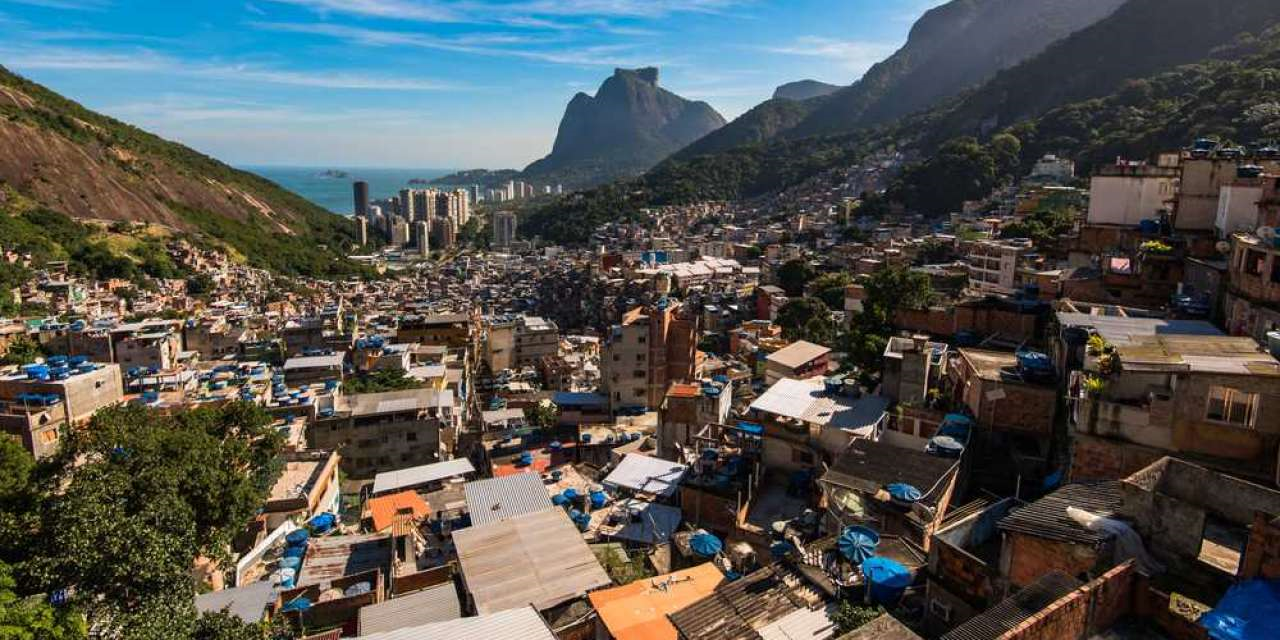
\includegraphics{C:/Users/Adelson/Desktop/thesis/subindo/family_medicine_impact/livro/rocinha.png}

\hypertarget{intro}{%
\chapter{Introduction}\label{intro}}

\begin{verbatim}
Mas eu ainda espero angariar as simpatias da opinião, 
e o primeiro remédio é fugir a um prólogo explícito e longo.
\end{verbatim}

Perguntar se investimento em educação é benéfico para a sociedade pode parecer algo obsoleto e desnecessário. Qualquer pessoa com o mínimo de instrução e bom senso concordaria que educação é um dos pilares que estruturam as sociedades e que investir recursos financeiros nesta área é fundamental para o seu desenvolvimento. Essas afirmações fazem parte da retórica política corrente e aparentemente não há discordância quanto à importância da universalização da alfabetização, da aquisição de conhecimentos gerais, do desenvolvimento de habilidades matemáticas, do conhecimento de história, geografia e ciências. Contudo, há uma série de fatos históricos, políticos e econômicos que tornam a discussão sobre ensino médico e treinamento de especialidades uma questão um pouco mais complexa do que se pode supor.

Apesar de ter o primeiro programa de residência iniciado em 1944 no Brasil, a regulamentação desta forma de curso de pós-graduação latu sensu veio a acontecer somente em 19771 a partir do decreto nº 80.281 que criava a Comissão Nacional de Residências Médicas (CNRM) e estabelecia que os programas de residência médica seriam caracterizados por ``treinamento em serviço, em regime de dedicação exclusiva, funcionando em Instituições de saúde, universitárias ou não, sob a orientação de profissionais médicos de elevada qualificação ética e profissional'' e que teriam duração mínima de um ano, contemplando 1.800 horas de atividade assistencial, sendo quatro horas semanais dedicadas a atividades de teóricas não assistenciais2. Isso ocorreu antes do estabelecimento do Sistema Único de Saúde3 (SUS) e antes mesmo do estabelecimento da Medicina de Família ser reconhecida como especialidade médica, fato que ocorreu em 1981 ainda sob o nome de Medicina Geral e Comunitária4.

Apesar do aumento recente na oferta de vagas para residência médica no Brasil impulsionado pelo pelo Programa PróResidência5 que aumentou a oferta de vagas em áreas prioritárias do país, em 2017 havia somente 16.499 vagas ofertadas para um contingente de 18.753 novos médicos formados6. Além de oferta ainda limitada de vagas para atender à demanda de médicos recém-formados, há também problemas quanto à distribuição destas vagas de acordo com as especialidades médicas, sendo a Atenção Primária à Saúde (APS) a área mais sensível à esta distribuição desigual. Por ser um nível de atenção à saúde ainda em construção no Brasil, apresenta uma demanda enorme de Médicos de Família e Comunidade treinados e capacitados, porém apenas 4,4\% das vagas atuais de residência são destinadas a esta especialidade7.

Formação médica especializada no formato de residência médica, ainda não é universal para todos os alunos graduados em escolas médicas no Brasil e comumente um aluno recém formado pode não conseguir uma vaga de residência na especialidade escolhida mesmo prestando prova para diversos programas. Ao mesmo tempo em que vários médicos recém-formados ficam de fora de programas de residência médica pela falta de vagas, a legislação brasileira permite ao médico trabalhar e exercer procedimentos específicos mesmo sem nenhuma especialização formal e reconhecida8,9. Isto é algo que aproxima o Brasil a outros países de baixa e média renda quanto a governança e regulação e o afasta daqueles onde a APS encontra-se madura nos quais uma grande parte das vagas são destinadas para Medicina de Família.

Dentro de um cenário hospitalar, em um ambiente cirúrgico, dificilmente um cirurgião sem especialização em cirurgia cardíaca seria contratado para realizar uma valvuloplastia, por exemplo, mas não é incomum que médicos sem treinamento exerçam a função de emergencistas -- função comumente exercida por médicos recém-formados no Brasil e que não recebe a mesma importância dada em alguns países desenvolvidos. Neste contexto, as forças que orientam e regulam a oferta de vagas em residência médica, os tipos de especialidades que serão privilegiadas e os locais de aberturas de novas vagas de residência não são orientadas exclusivamente visando atender às demandas de saúde da população, mas recebem grande influência de grupos políticos de especialidades e corporações médicas2.

Apesar da falta de regulação e de planejamento estratégico na formação médica especializada para atender às demandas em saúde da população e de termos uma desigualdade enorme na densidade de médicos no país, concentrando especialistas nos grandes centros urbanos e áreas mais ricas, as políticas de incentivo para a criação de novas vagas de residência médica privilegiaram a MFC, aumentando de 1,4\% para 4,4\% das vagas ofertadas no país6. Mesmo assim, a proporção de vagas de residência em MFC no Brasil ainda é muito menor do que o encontrado em países como Canadá, Espanha e Inglaterra, onde metade do total de vagas é destinado à MFC10. Isso deixa o Brasil muito distante de alcançar a meta regional estabelecida pela Organização Panamericana de Saúde de que 40\% da força laboral deve estar concentrada na APS11. A obrigatoriedade de cursar um programa de residência para se exercer a medicina ainda está longe de se tornar uma realidade no Brasil, fazendo com que provimento, fixação e desenvolvimento de competências clínicas - três objetivos principais da formação médica especializada - continuem sendo metas muito longe de serem alcançadas2.

Nos seus quase 30 anos de história o Sistema Único de Saúde (SUS), com suas diretrizes de universalidade, integralidade do cuidado, participação popular, resolutividade e equidade3, conseguiu avanços importantes ao ampliar acesso a serviços e garantindo direito ao cuidado em saúde. Contudo, muito ainda precisa ser feito para que seja considerado um sistema de saúde robusto e verdadeiramente universal, principalmente minimizando desigualdades em saúde entre regiões ricas e pobres do país12.

Além das dificuldades históricas de desenvolvimento do sistema de saúde, eventos recentes trazem uma ameaça séria à sustentabilidade do SUS, a partir da implementação das políticas de austeridade propostas durante os anos de governo de Michel Temer13, colocando em risco conquistas importantes alcançadas durante sua história, como ampliação da APS, aumento da cobertura de serviços, redução da mortalidade infantil14 e da mortalidade por doenças crônicas não transmissíveis (DCNT)15. Com a implementação das políticas de austeridade e com o previsto congelamento de investimentos na área da saúde e educação pelos próximos 20 anos há expectativa de uma redução na diminuição da taxa de mortalidade infantil, fazendo com que o país reduza os ganhos que seriam esperados em saúde caso os investimentos fossem mantidos16.

Historicamente algumas iniciativas buscaram minimizar essas desigualdades de acesso a serviços e a primeira estratégia nacional voltada para a atenção primária à saúde (APS) foi o Programa de Saúde da Família (PSF) que, desde sua concepção em 1991 e implementação em 199417, ampliou gradativamente sua cobertura de população assistida, chegando a 56\% de cobertura em 201318, e a 64\% em 201619. Esta iniciativa teve impactos substanciais sobre a saúde da população brasileira, principalmente na redução da mortalidade infantil20, na redução de internações hospitalares desnecessárias21 e na redução da mortalidade por doenças cardiovasculares22.

Contudo, não foi somente em indicadores de saúde pública que este programa teve efeito. A criação de novos postos de trabalho em unidades de APS teve também um efeito tanto no mercado de trabalho, ao aproximar novos médicos do trabalho na APS, impulsionando assim o crescimento da Sociedade Brasileira de Medicina de Família SBMFC), quanto na criação de um novo mercado de trabalho nos planos privados de saúde, que passaram a ver a MFC como uma forma de trazer os atributos da APS para seus seus serviços, reduzindo custos e trazendo melhores resultados no cuidado em saúde23,24.

\hypertarget{literature}{%
\chapter{Literature}\label{literature}}

Aqui já entra outro capítulo

\hypertarget{methods}{%
\chapter{Methods}\label{methods}}

We describe our methods in this chapter.

\hypertarget{applications}{%
\chapter{Applications}\label{applications}}

Some \emph{significant} applications are demonstrated in this chapter.

\hypertarget{example-one}{%
\section{Example one}\label{example-one}}

\hypertarget{example-two}{%
\section{Example two}\label{example-two}}

\hypertarget{final-words}{%
\chapter{Final Words}\label{final-words}}

We have finished a nice book.

\bibliography{book.bib,packages.bib}


\end{document}
